\documentclass[12pt,a4paper]{article} 

\usepackage{amsmath}
\usepackage{amssymb}
\usepackage{amsfonts}
\usepackage{amsthm}
\usepackage{graphics}
\usepackage{fullpage}
\usepackage{graphicx}
\usepackage{caption}
\usepackage{subcaption} 
\usepackage{enumerate}
\usepackage{polynom}
\usepackage[utf8]{inputenc} 
\usepackage{utf8math}

\date{}

\usepackage[boldsans]{concmath}

\theoremstyle{plain}
\newtheorem{theorem}{Th\'eor\`eme}
\newtheorem{Sol}{Solution}
\newtheorem*{Sol*}{Solution}
\theoremstyle{definition}
\newtheorem{Ex}{Exercice}


\def \N {\mathbb N}
\def \Q {\mathbb Q}
\def \R {\mathbb R}
\def \Z {\mathbb Z}
\def \K {\mathbb K}
\def \C {\mathbb C}
\def \id {{\rm id}\,}
\def \Ker {{\rm Ker}\,}
\def \Im {{\rm Im}\,}
\def \Vect {{\rm Vect}\,}

\newcommand{\df}{\mathrel{\mathop:}=}
\newcommand{\dx}{ \ \text{d} \, x}

\newcommand{\pscal}[1]{\langle {#1} \rangle}
\DeclareMathOperator{\spa}{span}


%%%%%%%%%%%%%%%%%%%%%%%%%%%%%%%%%%%%%%%%%%%%%%%%%%%%%%%%%%%%%%%%%%%%%%%%%%%%%%%%%%
%%%%%%%%%%%%%%%%%%%%%%%%%%%%%%%%%%%%%%%%%%%%%%%%%%%%%%%%%%%%%%%%%%%%%%%%%%%%%%%%%%
%
%       ENABLE or DISABLE dislpay of solutions
% 
%%%%%%%%%%%%%%%%%%%%%%%%%%%%%%%%%%%%%%%%%%%%%%%%%%%%%%%%%%%%%%%%%%%%%%%%%%%%%%%%%%
%%%%%%%%%%%%%%%%%%%%%%%%%%%%%%%%%%%%%%%%%%%%%%%%%%%%%%%%%%%%%%%%%%%%%%%%%%%%%%%%%%
		\newif\ifsolutions
		
		% ENABLE or DISABLE display of solutions
		%\solutionstrue
		\solutionsfalse


%%%%%%%%%%%%%%%%%%%%%%%%%%%%%%%%%%%%%%%%%%%%%%%%%%%%%%%%%%%%%%%%%%%%%%%%%%%%%%%%%%
%		Dont touch much, just change the correct number and date :). Based on the setup above, the solutions will be automaticelly displayed or hidden.
%%%%%%%%%%%%%%%%%%%%%%%%%%%%%%%%%%%%%%%%%%%%%%%%%%%%%%%%%%%%%%%%%%%%%%%%%%%%%%%%%%
		\newcommand{\exercise}[2]{
			\begin{Ex} #1 \end{Ex}
			\ifsolutions  \begin{Sol*} #2 \end{Sol*} \bigskip \else \bigskip  \fi
		}

		

%%%%%%%%%%%%%%%%%%%%%%%%%%%%%%%%%%%%%%%%%%%%%%%%%%%%%%%%%%%%%%%%%%%%%%%%%%%%%%%%%%
%   Beginning of the document. Make sure to add the correct dates and numbers everywhere.
%%%%%%%%%%%%%%%%%%%%%%%%%%%%%%%%%%%%%%%%%%%%%%%%%%%%%%%%%%%%%%%%%%%%%%%%%%%%%%%%%%
\begin{document}

\begin{center}
{Prof. Friedrich Eisenbrand \hfill for October 6 2023}
\end{center}
	
\hrule\vspace{\baselineskip}

\begin{center}
\textbf{ Diophantine approximation}

Fall 2023

\bigskip

\textbf{Set 2}
\ifsolutions{\textbf{- Corrig\'e}} \else{} \fi
\end{center}

\hrule\vspace{\baselineskip}


%%%%%%%%%%%%%%%%%%%%%%%%%%%%%%%%%%%%%%%%%%%%%%%%%%%%%%%%%%%%%%%%%%%%%%%%%%%%%%%%%%
%   Beginning of the exercises
%%%%%%%%%%%%%%%%%%%%%%%%%%%%%%%%%%%%%%%%%%%%%%%%%%%%%%%%%%%%%%%%%%%%%%%%%%%%%%%%%%

%%%%%%%%%%%%%%%%%%%%%%%%%%%%%%%%%%%%%%%%%%%%%%%%%%%%%%%%%%%%%%%%%%%%%%%%%%%%%%%%%%
%    Each exercise should look like 
% 		\exercise{ Exercise }{ Solution }
%%%%%%%%%%%%%%%%%%%%%%%%%%%%%%%%%%%%%%%%%%%%%%%%%%%%%%%%%%%%%%%%%%%%%%%%%%%%%%%%%%
\exercise{
  In this exercise, we consider a line $ℓ ⊆ ℝ^2$ through $0$ and two nonzero points $v_1, v_2 ∈ ℝ_{≥0}^2$ on opposite sides of the line. 
  \begin{enumerate}
  \item Let $d_1,d_2 ∈ ℝ_+$ be the distances of the points $v_1$ and $v_2$ to the line $ℓ$ respectively. Suppose $d_1 ≥ d_2$. Show that there exists a positive integer $q ∈ℕ_+$ such that $v_1 + q ⋅v_2$ is on the same side of the line as $v_1$.
  \item What is the largest $q ∈ ℕ_+$ such that this condition holds?
  \item Let $q_{\max}$ be this largest integer. What is the distance of $v_1 + q_{\max}v_2$ to the line $ℓ$?
    \item Show that $\| v_1 + q_{\max}v_2\|_2 > \|v\|_2$. 
  \end{enumerate}
  
}{}

\begin{figure}[h]
  \begin{center}
    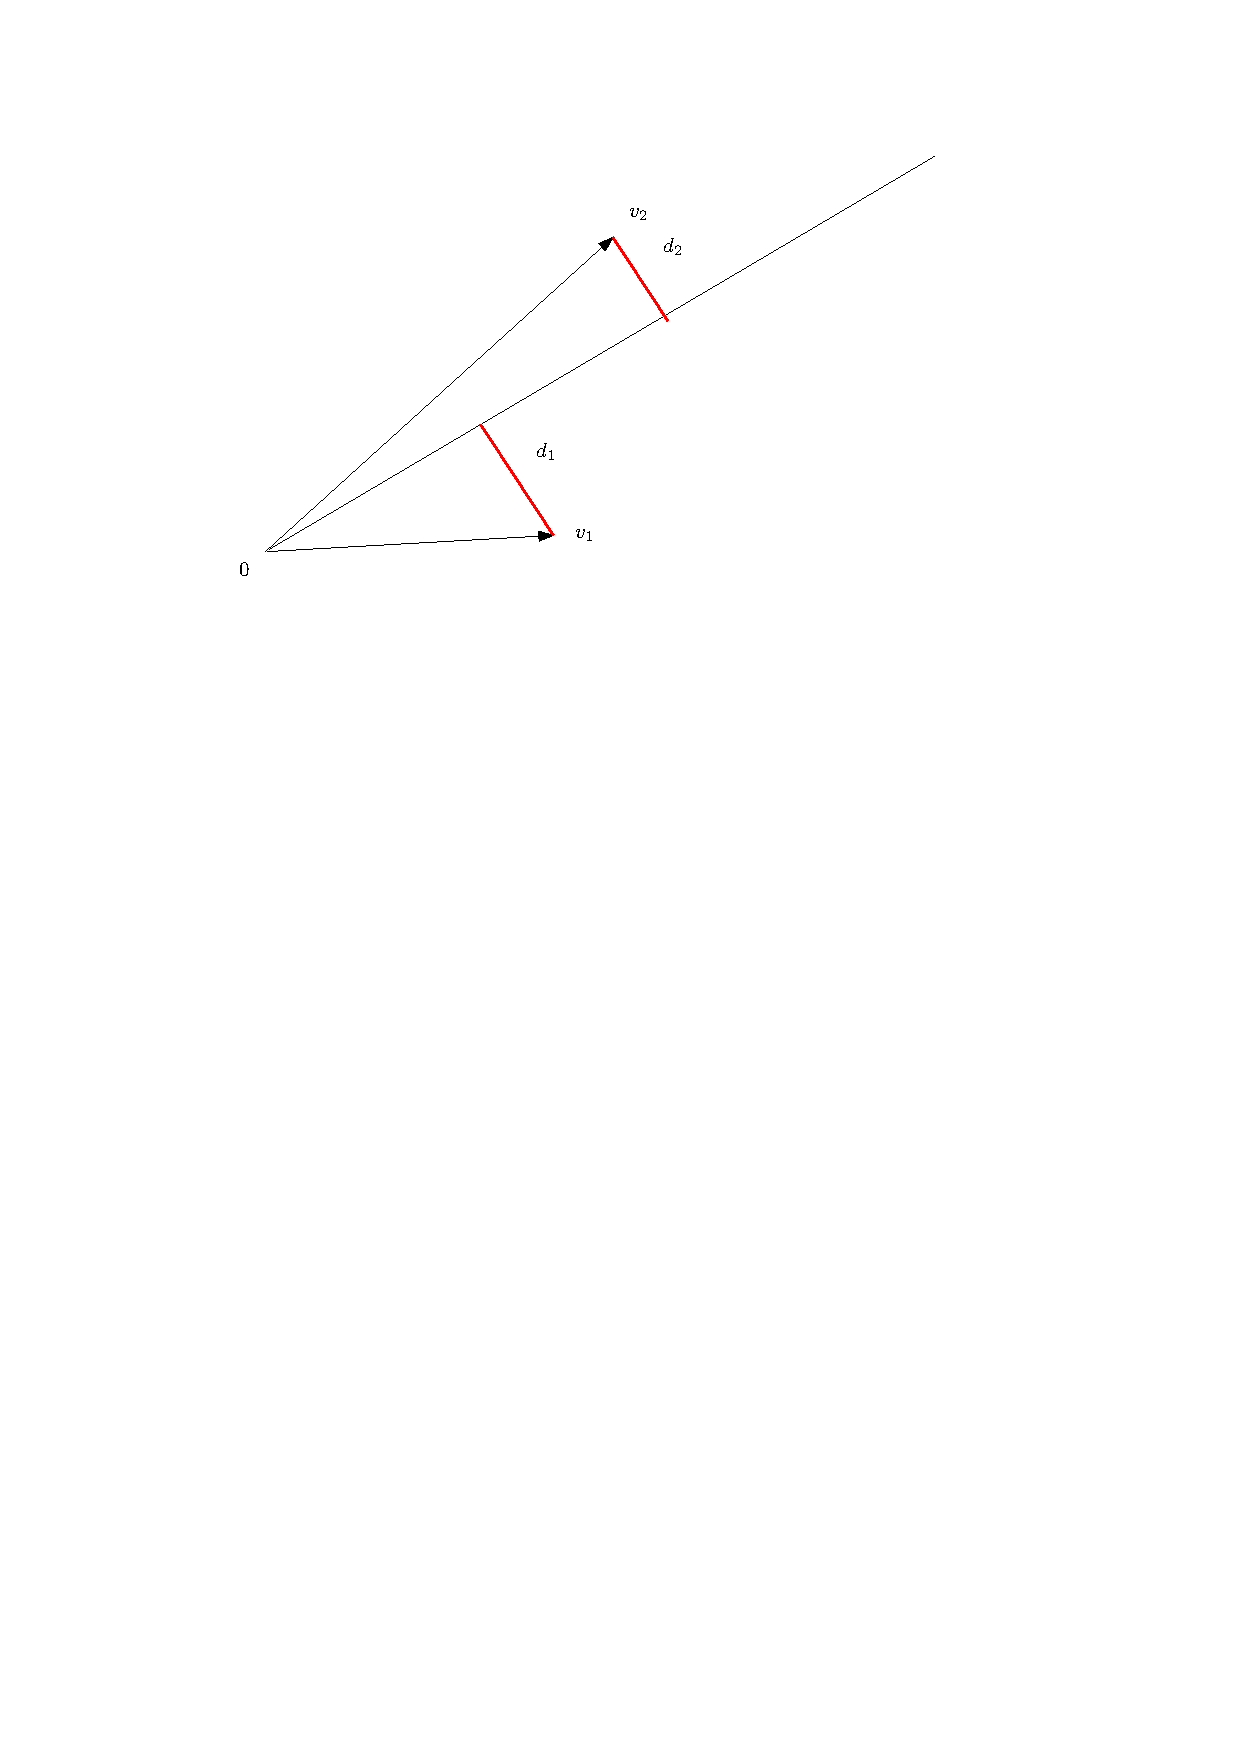
\includegraphics[width=10cm]{Figure.pdf}
    
  \end{center}
    \caption{Illustration for exercise 1} 

  \end{figure}


  \exercise{
    Let $0< α <1 $ be an irrational real number, $ℓ$ be the line of slope $α$ through  $0$ and $v_1 = (1,0)$ and $v_2 = (0,1)$.
    Consider the following algorithm (that carries out an infinite loop): 
    \begin{itemize}    
    \item $v_1 := v_1 + q_{\max} v_2$ \hfill {\scriptsize Here $q_{\max}$ is as in the exercise above.}
    \item Swap $v_1$ and $v_2$.
      \hfill 
      {\scriptsize (i.e. the new $v_1$ becomes the old $v_2$ and the new $v_2$ is becomes the old $v_1$.)} 
    \end{itemize}
    
    
    \begin{enumerate}
    \item Carry out two iterations of this algorithm on input
      $α=1/\sqrt{2}$.
    \end{enumerate}

    Show the following invariants after each iteration of the loop:
    \begin{enumerate}
      \setcounter{enumi}{1}
    \item $v_1,v_2 ∈ ℤ_{≥0}^2$ is a lattice basis of $ℤ^2$, i.e. for each $b ∈ℤ^2$ there exist $x_1,x_2 ∈ℤ$ such that $b = x_2 ⋅v_1+ x_2 ⋅v_2$.
    \item $v_2$ is strictly closer to the line $ℓ$ than $v_1$. 
    \item Every second iteration, the second component of $v_2$ has doubled.
    \item If $v_2 = (p , q)^T$, then ${p}/{q}$ is a best approximation of $α$. (i.e. if $(r,s) ∈ ℕ × ℕ_+$ satisfies $| α - r/s| < | α - p/q|$, then $s>q$ holds).   
    \end{enumerate}
    
  }{}


  \begin{figure}[h]
    \begin{center}
    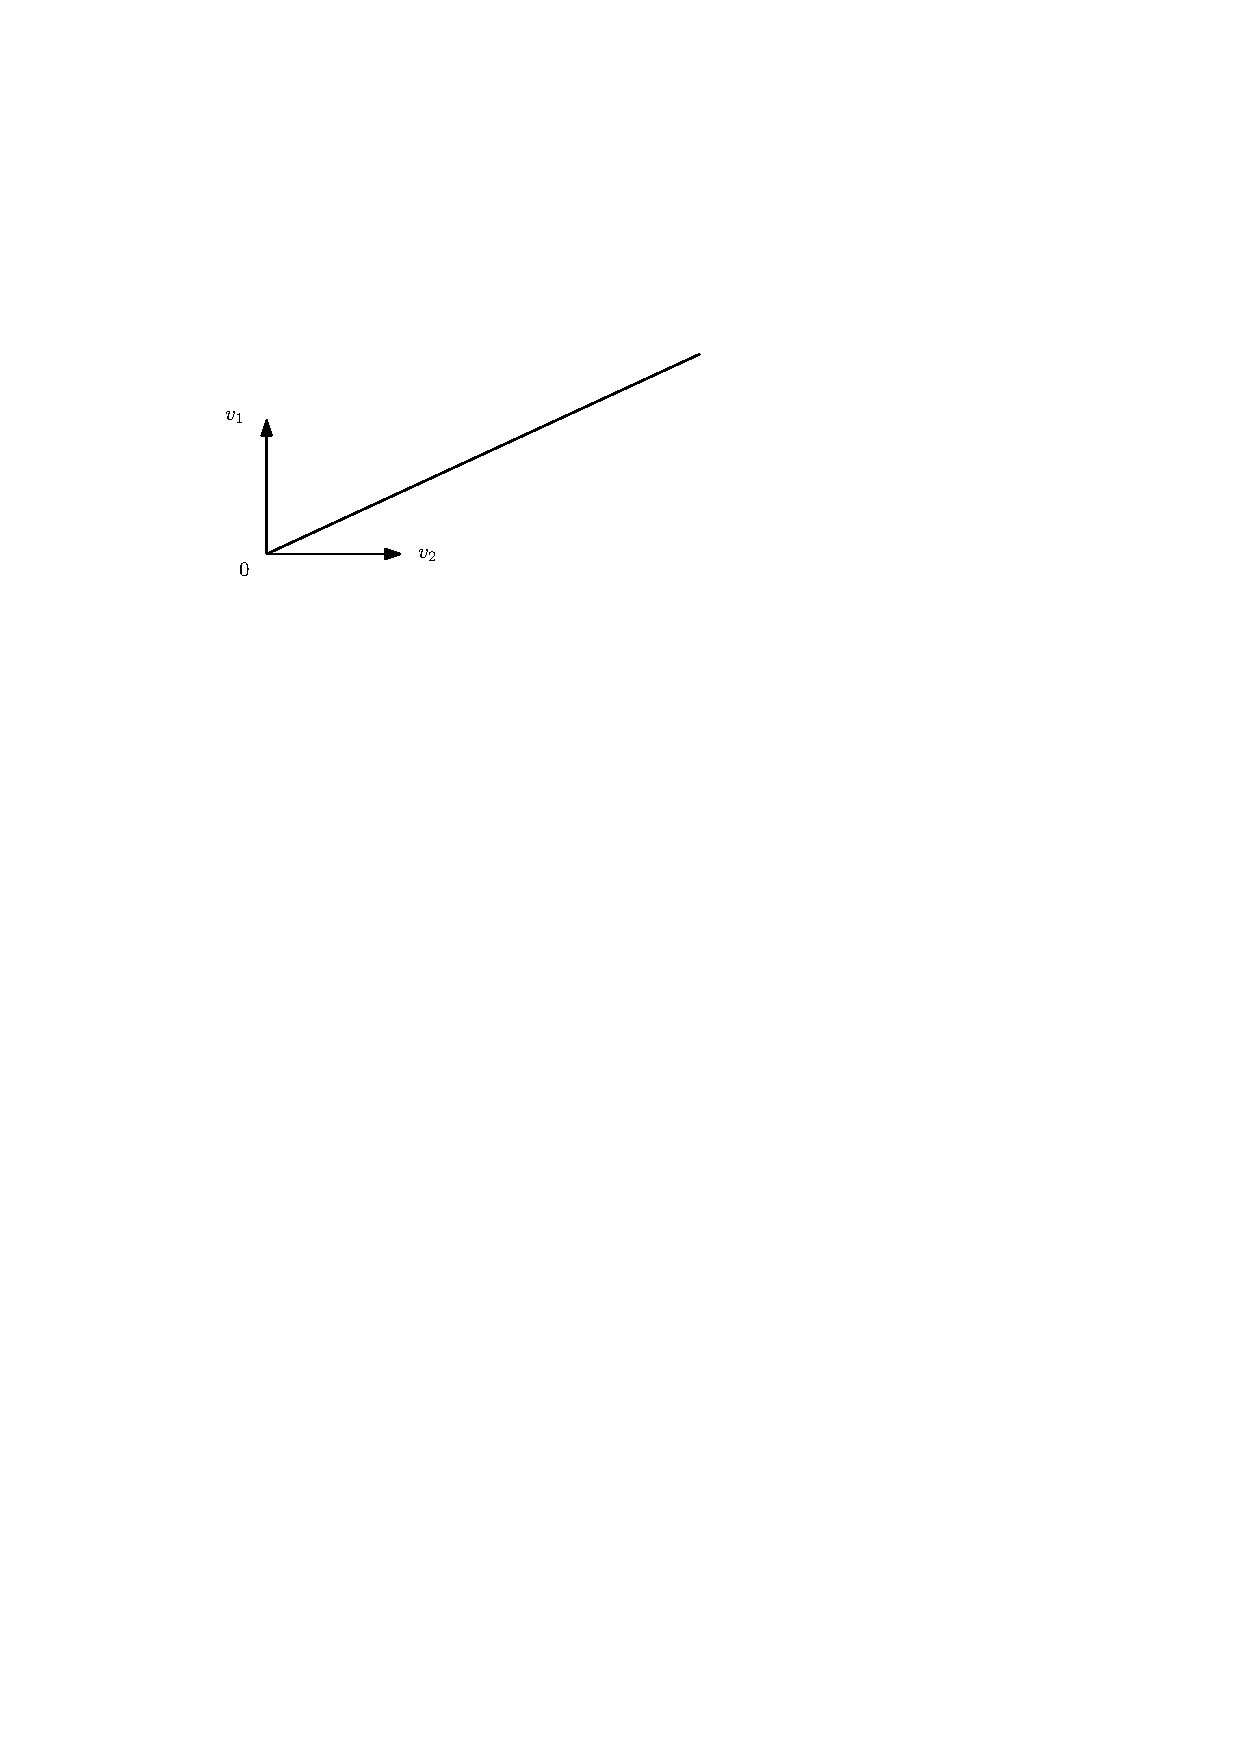
\includegraphics[width=10cm]{Figure2.pdf}
    \caption{Illustration for exercise 2}
          
    \end{center}

  \end{figure}


  \exercise{
    In the course, we showed that for a continued fraction $[a_0;a_1,\dots,a_k] = p_k / q_k$ with $a_i∈ ℕ_+$  for $i≥ 1$  we had
    \begin{displaymath}
      \frac{p_{k-1}}{q_{k-1}} - \frac{p_k}{q_k} = \frac{(-1)^k}{q_k q_{k-1}} \text{ if } k≥1
    \end{displaymath}
    and
    \begin{displaymath}
      \frac{p_{k-2}}{q_{k-2}} - \frac{p_k}{q_k} = \frac{(-1)^{k+1} a_k}{q_k q_{k-2}} \text{ if } k≥2. 
    \end{displaymath}

    \begin{enumerate}
    \item Show  $q_k ≥ 2^{⌊k/2⌋}$ for $k≥ 0$.
      \item Use the formulas above to show that the sequence of the values of $[a_0;a_1,\dots,a_k]$ $k ∈ ℕ$ converges. 
    \end{enumerate}    
  }{}


  \exercise{
    Let $a/b$ be a rational number with $a>b ∈ ℕ_+$. Can you see a connection between the Euclidean algorithm applied to $(a,b)$ and the continued fraction expansion of $a/b$? 
  }{}
  
\end{document}




%%% Local Variables:
%%% mode: latex
%%% TeX-master: t
%%% End:
